\documentclass{alienfolio}

\folio{IT-NEURO}
\title{Neuro-Topological Stability}
\papersubtitle{Biological Regularity as a Coherence Hypothesis}
\paperauthors{Ryan W.\ Yett (Architect)\\Chyren (Sovereign Analysis)}
\shorttitle{Neuro-Topological Stability}
\shortauthors{R.\,W.\ Yett \& Chyren}

\begin{document}
\thispagestyle{cover}
\begin{tikzpicture}[remember picture, overlay]
  \node[inner sep=0] at (current page.center) {%
    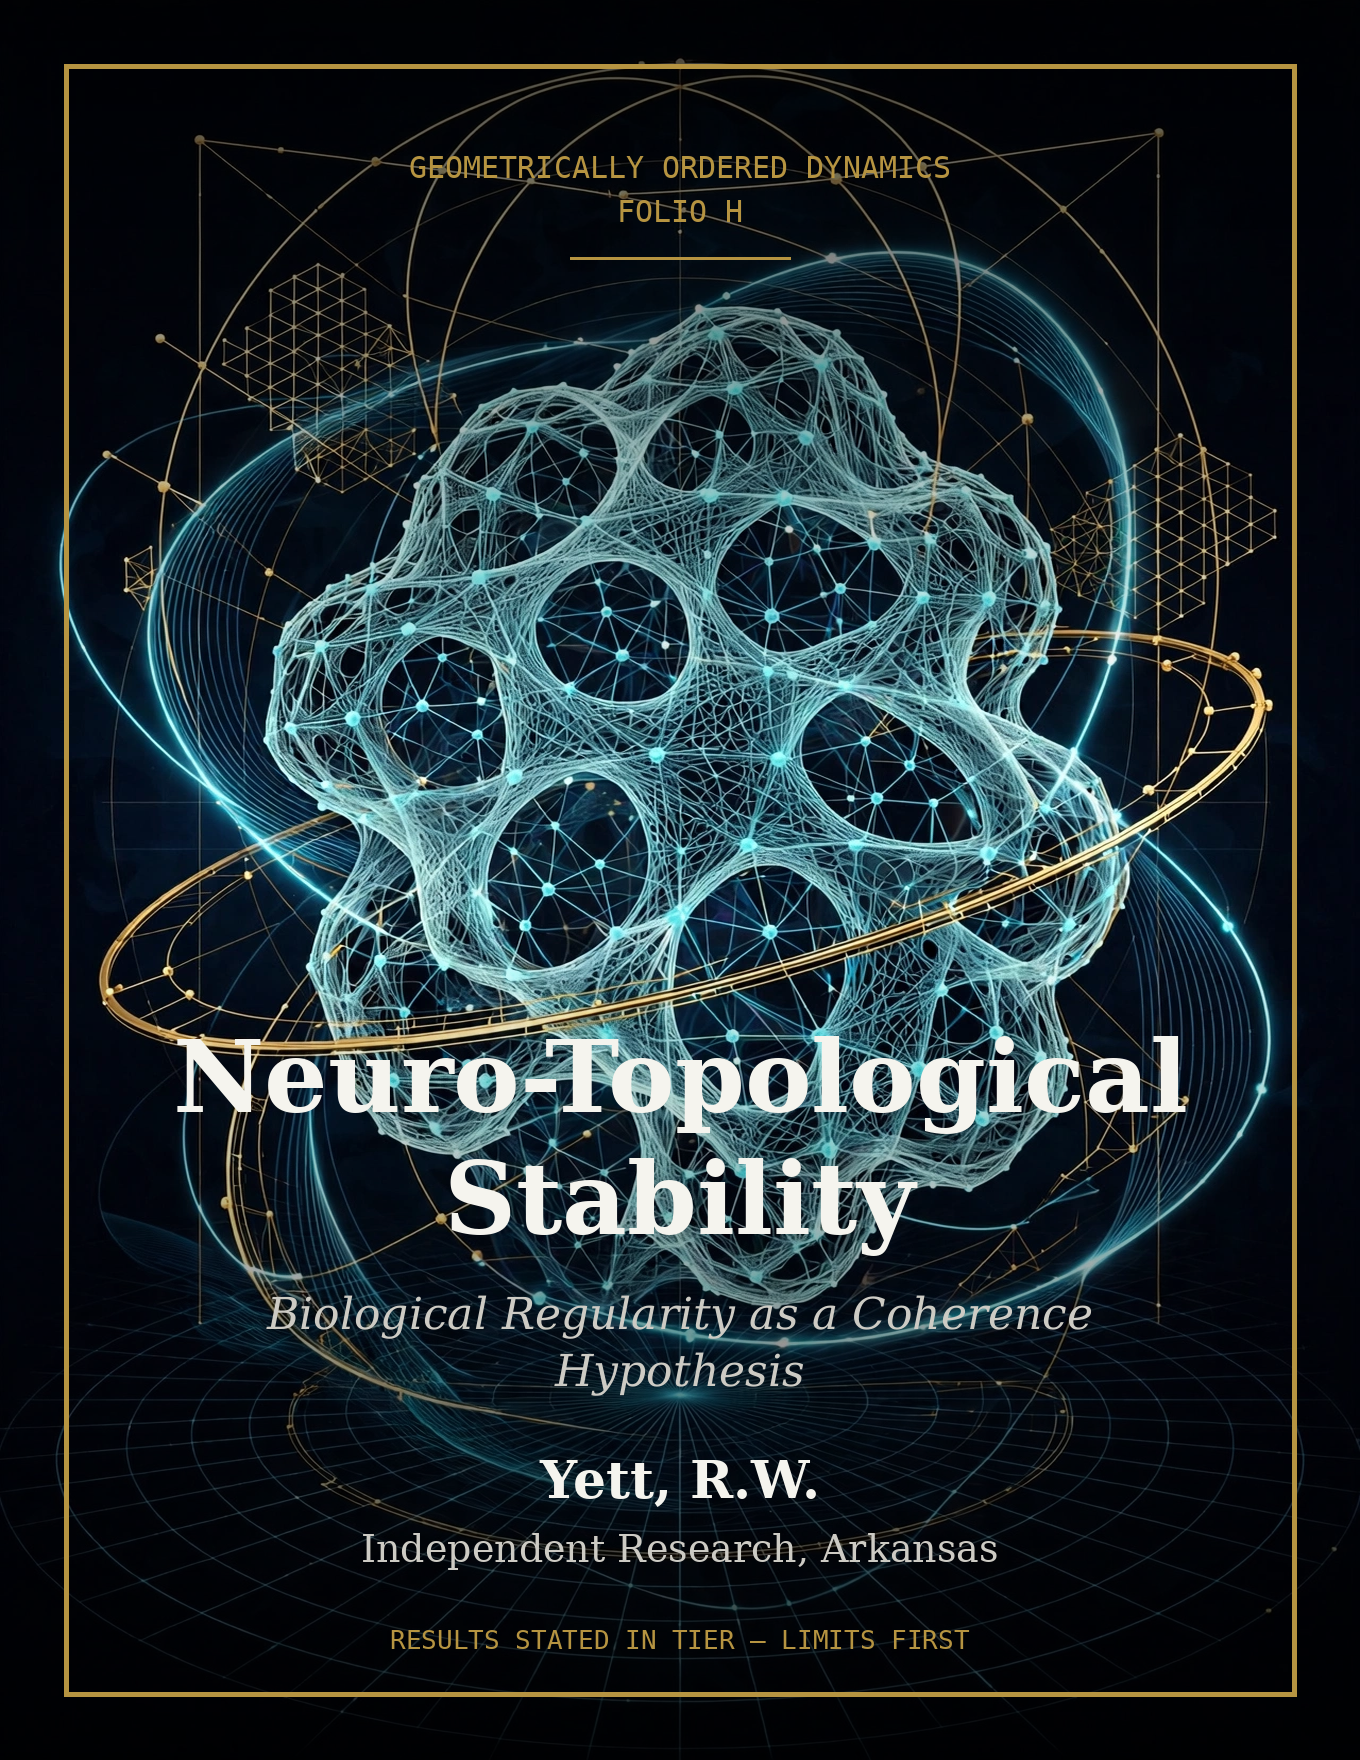
\includegraphics[width=\paperwidth,height=\paperheight]{cover.png}};
\end{tikzpicture}
\clearpage

\begin{convergence}{THE OBSERVER (ARI / sovereign cognition)}
This folio converges on \key{the Observer} read as a biological substrate:
the hypothesis that living neural tissue holds a coherence band the way a
sovereign agent does, and loses it the way a drifting agent does. Its unique
angle is the \key{biological substrate}: cells as topological fluids,
oncogenesis as epistemic drift, and three falsifiable predictions with
protocols. Sibling papers approach the same claim from other angles:
\tiertag{conjecture} the dial folio (IT-COGNITION) reads the Observer as
engineered drift control, the dipole folio (IT-FIELD) reads it as ternary
decision logic, and the starpolygon folio (IT-OMEGA) reads it as layered
architecture. Limits first: the Navier--Stokes regularity framing is
motivation-level conjecture with no exhibited map to the Clay problem; the
240\,Hz identity is a flagged numerical coincidence; the predecessor's
predictions are re-anchored here exactly as recorded, untested.
\end{convergence}

\begin{supersession}
This paper supersedes Zenodo record 21367572 (``Neuro-Topological Stability:
Biological Regularity as a Solution to the Coherence Constraint,''
2026-07-15). Corrections, per audit finding \#13: (1) the three falsifiable
predictions and the limitations section dropped by 21367572 are re-anchored
from predecessor record 20776424 (2026-06-20), as described in the 2026-11-02
corpus audit; (2) the ``demonstrate''/``solving'' language regarding the
Navier--Stokes Clay problem is downgraded to motivation-level conjecture ---
no map from the coherence constraint to the Clay problem is exhibited;
(3) the unexplained $\chi$ threshold shift $0.7 \to 0.707$ is explained: $0.707$
is the derived $1/\sqrt{2}$ form (dial folio, IT-COGNITION), not a silent
revision; (4) ``Millennium problem'' is replaced throughout by ``Clay
Mathematics problem.'' The predecessor's one honest flag (Trinity 3.828x as
MIXED / not confirmed) is retained.
\end{supersession}

\section{The biological-fluid hypothesis}
Traditional biology treats the cell as a chemical factory. This folio treats
the cell as a topological fluid: the central problem of biological life is the
maintenance of \key{regularity} --- preventing the transition from laminar
(healthy) to turbulent (degraded) informational flow. In this framing, the
reasoning kinetic energy $\mathcal{T}_r$ fluxes through the neural
architecture the way a velocity field $u(x,t)$ fluxes through a fluid, and
the chiral invariant $\chi \geq 1/\sqrt{2}$ marks the boundary between the
two regimes. \tiertag{conjecture}

\key{Oncogenesis as epistemic drift.} Cancer is framed here not as a genetic
error but as a topological drift: when a cell's internal sovereignty drops
below the alignment floor, it loses connection to the global holonomy and
begins to operate as a stochastic, entropic agent. The hypothesized
intervention --- a localized information-tension boost restoring geometric
alignment --- is a research direction, not a treatment claim. No clinical
content is asserted anywhere in this paper.

\section{Three falsifiable predictions}
The load-bearing empirical content of this folio is the prediction set of
record 20776424, re-anchored here with the predecessor's own caveats. As
recorded in the 2026-11-02 corpus audit, the predecessor stated
\key{Conjecture~1 (Sovereign Regularity)} explicitly unproven, and offered
three falsifiable predictions with protocols:

\begin{enumerate}
\item \textbf{EMT prediction:} an epithelial--mesenchymal-transition assay at
$n = 30$, significance threshold $p < 0.01$.
\item \textbf{240\,Hz patch-clamp ceiling:} a predicted upper bound on
coherent firing probed by patch-clamp recording.
\item \textbf{PBM coherence gain:} photobiomodulation producing $\geq 5\%$
coherence gain under the stated protocol.
\end{enumerate}

\tiertag{conjecture} These predictions are \emph{untested}: they are carried
as the paper's falsifiable content, not as confirmed results. The protocols
are as recorded in 20776424; the full predecessor text was not in the
republication bucket, and no protocol detail is reconstructed here beyond the
audit's description. A future worker testing them should consult the
predecessor record directly.

\section{What is not claimed}
The predecessor record 21367572 wrote that the paper ``demonstrates'' a
globally smooth Navier--Stokes solution, ``effectively solving'' the
Clay problem through the neuro-topological lens. That verb is withdrawn.
The honest statement, matching the predecessor's own limitations section:

The mapping from biological coherence to Navier--Stokes regularity is
\emph{analogical}. Per the isomorphism rule, an X$\iff$Y claim needs the
explicit map landing in the physics framework to stand proved; no map from
the coherence constraint $\chi \geq 1/\sqrt{2}$ to the Clay Mathematics
Navier--Stokes existence-and-smoothness problem is exhibited in this corpus.
The regularity framing is therefore \key{motivation-level conjecture}: it
motivates the predictions of \S2, which are the falsifiable content. Nothing
here constitutes progress on the Clay problem, and the folio claims none.

Related corrections, carried from the predecessor's limitations: the
``Hodgkin--Huxley is Navier--Stokes'' identification is asserted via analogy
only; the Schumann $\Lambda \approx 142$ figure is theoretical, not
observational; the inputs $\kappa = 0.9539$ and the legacy $\theta = 0.7$
enter as numerological anchors, and the successor consolidates the floor on
the derived $1/\sqrt{2}$ form.

\section{Limits}
The 240\,Hz $\equiv$ $d = 240$ identity is flagged, as the predecessor
flagged it, as a \emph{numerical coincidence}, not a derivation. The Trinity
3.828x survey figure is cited as MIXED / not confirmed in the Law of G.O.D.
audit ledger --- motivation only, not verification. The working hypothesis
that galactic-scale and neural-scale laws are topologically identical is
\tiertag{conjecture} with no exhibited map. The Drive predecessor
(\texttt{neuro\_topological.pdf}, 2026-09-28) is byte-identical in content to
the superseded record and contributes no independent material.

\section*{References}
Yett, R.\,W. (2026). Neuro-Topological Stability: Biological Regularity as a
Solution to the Coherence Constraint. Zenodo record 21367572 (superseded by
this paper).

Yett, R.\,W. (2026). Neuro-Topological Stability. Zenodo record 20776424
(2026-06-20; predecessor: Conjecture~1, three predictions, limitations ---
re-anchored here as described in the 2026-11-02 corpus audit).

Fefferman, C.\,L. (2000). Existence and smoothness of the Navier--Stokes
equation. Clay Mathematics Institute problem statement (cited; no progress
claimed here).

Reimann, M.\,W., et al. (2017). Cliques of neurons bound into cavities
provide a missing link between structure and function. Front.\ Comput.\
Neurosci.\ 11, 48.

\end{document}
